
%  The lines beginning with "%" are comments. 
%  Theses comments explain how to use this template for
%  preparing the Seminar report. 
%
%  The first non-comment line below contain the matter that
%  go into the preamble of the input file. These are collected in a 
%  file by name "preamble.tex". This file can be seen in the 
%  folder "SeminarReportTemplate". 
%
%  Do not make any changes in the first non-comment line below.
%
\documentclass[11pt, twoside]{book}
\let\cleardoublepage\clearpage
\usepackage{graphicx, fancyhdr, amsmath,times, url}
\setlength{\oddsidemargin}{3cm}
\newcommand{\VAtitle}[1]{\def\vtitle{Bitcoin: A Cryptocurrency}}
\newcommand{\VAauthor}[1]{\def\vauthor{Savitha K J}}% Write full name without, repeat without, Mr. or Ms.
\newcommand{\VAadmissionyear}[1]{\def\vadmissionyear{2010}}
\newcommand{\VAregisternumber}[1]{\def\vregisternumber{VEAKECS049}}% Write University Examination Register Number.
\newcommand{\VAguide}[1]{\def\vguide{Ms. Geethu P C M.Tech, MISTE}}% Write full name with Mr. or Ms. or Dr. or Prof.
\newcommand{\VAhod}[1]{\def\vhod{Col MP Induchudan,  M.E., FITE}}% Write full name with Mr. or Ms. or Dr. or Prof. 
%
%
%  No changes in the next non-comment line also.
%
\begin{document}
%
%***************************************************
%
%  In the next line, replace "Seminar Title" by the title of your seminar.
%
\VAtitle{Seminar Title}%
%
%  In the next line, replace "Student" by your name. 
%  Write full name without, repeat without, Mr. or Ms.
%
\VAauthor{Student}%
%
%  In the next line, replace "2008" by the year of your admission 
%  to the College.
%
\VAadmissionyear{2010}%
%
%  In the next line, replace "VExxMCAnnn" by your 
%  University Examination Register Number.
%
\VAregisternumber{VExxxCSnnn}% 
%
%  In the next line, replace "Guide" by the full name of your guide or supervisor 
%  with Mr. or Ms. or Dr. or Prof.
%
\VAguide{Guide}% 
%
%  In the next line, replace "hod" by the full name of Head of Department 
%  with Mr. or Ms. or Dr. or Prof.
\VAhod{hod}
%
%  Printing the first few pages: title, certificate, acknowledgement, etc.
%  No changes in the next non-comment line.
%
%
\makeatletter
\renewcommand{\chapter}{\if@openright\cleardoublepage\else\clearpage\fi
                    %\thispagestyle{fancy}%
                    \global\@topnum\z@
                    \@afterindentfalse
                    \secdef\@chapter\@schapter}%
%
\makeatother
%
\pagestyle{empty}
%\frontmatter
%
%******************************************************
%
\begin{titlepage}
\newcommand{\HRule}{\rule{\linewidth}{0.5mm}}
\begin{center}
% Upper part of the page
% Title
%\quad\\[0.3cm]
{\large \sffamily CS 09 805 (P) : Seminar}\\[0.2cm]
\HRule \\[0.5cm]
{ \huge\sffamily \bfseries \vtitle}\\[0.2cm]
\HRule \\[5.20cm]
% Author
{\Large \sffamily\bfseries  \vauthor}\\
{\large \sffamily Reg. No. \vregisternumber\\ 
S8 CSE (\vadmissionyear\ Admissions)} \\[4cm] 
% Bottom of the page
%\vfill

\includegraphics[width=0.40\textwidth]{VidyaLogo}\\[0.2cm]
{\Large \sffamily\bfseries Department of Computer Science and Engineering}\\ {\large\sffamily Vidya Academy of Science \& Technology\\ \normalsize Thalakkottukara, Thrissur - 680 501}\\
({\tt http://www.vidyaacdemy.ac.in})\\
\end{center}
\end{titlepage}
%
%******************************************************
%

%%
%******************************************************
%
\begin{titlepage}
\newcommand{\HRule}{\rule{\linewidth}{0.5mm}}
\begin{center}
% Upper part of the page
% Title
%\quad\\[0.3cm]
{\large \sffamily CS 09 805 (P) : Seminar}\\[1cm]
%\HRule \\[0.5cm]
{ \huge\sffamily \bfseries \vtitle}\\[5.9cm]
% Author
{\Large \sffamily \bfseries \vauthor}\\
{\large \sf  Reg. No. \vregisternumber\\ 
S8 CSE (\vadmissionyear\  Admissions)} \\[4cm] 
% Bottom of the page
%\vfill

\includegraphics[width=0.40\textwidth]{VidyaLogo}\\[0.2cm]
{\Large \sffamily \bfseries Department of Computer Science and Engineering}\\ {\large \sffamily Vidya Academy of Science \& Technology\\ \normalsize Thalakkottukara, Thrissur - 680 501}\\
({ \bf \tt http://www.vidyaacademy.ac.in})\\[1cm]
\end{center}
\end{titlepage}
%
%******************************************************
%
\clearpage
\pagenumbering{roman}
%
\addcontentsline{toc}{chapter}{\quad Certificate}
%
\begin{center}
\hrule
\quad\\[0.75cm]
{\Large \bf Department of Computer Science and Technology}\\
{\large \bf Vidya Academy of Science \& Technology}\\
{\normalsize \bf Thalakkottukara, Thrissur - 680 501\\
({\tt http://www.vidyaacademy.ac.in})}\\[0.5cm]

\includegraphics{VidyaLogo}\\[1.25cm]
%
{\Large \bf CERTIFICATE}\\[1cm]
%
\end{center}
\index{certificate}
\index{University of Calicut}
This is to certify that the report titled 
{\bf \vtitle} is a bona-fide record of the 
Seminar presented by {\bf \vauthor\  
(Reg. No. \vregisternumber)}    of the Eighth 
Semester B.Tech CSE (\vadmissionyear\ admissions) 
of Vidya Academy of Science \& Technology, 
Thrissur - 680 501 in partial fulfilment of the 
requirement for the award of the Bachelor of Technology in Computer Science and Engineering from the University of 
Calicut.\\[0.1cm]
%
\begin{center}
\begin{tabular}{llll}
\multicolumn{2}{l}{\bf Seminar Guide}    
&\multicolumn{2}{l}{\bf Head of Department}   \\
   & & \\
Name: &&  Name: \\
\vguide\ && \vhod\ \\ \\
Signature: \quad  ................................
\qquad \qquad && Signature: \quad 
................................ \\
& & & \\
Date: \hspace{10mm} \today & & Date: \hspace{10mm} \today \\
\end{tabular}
\\[1cm]
{\small (Seal of Department of Computer Science and Engineering)}
\quad \\[0.75cm]
\hrule
\end{center} 
%
\vspace*{\fill}
%
\clearpage
\pagestyle{fancy}
\lhead{{\small \vtitle}} \rhead{\thepage}
\lfoot{{\scriptsize Department of Computer Science \& Engineering, 
Vidya Academy of Science \& Technology, Thrissur}}
\rfoot{
\includegraphics[width=0.5cm]{VidyaLogo}}
\cfoot{ }
%
\renewcommand{\headrulewidth}{1pt}
\renewcommand{\footrulewidth}{0.5pt}
%
%\clearpage
\thispagestyle{fancy}
%
\addcontentsline{toc}{chapter}{\quad Acknowledgement}
%
\chapter*{Acknowledgement}
%
\index{acknowledgment}
I wish to record my indebtedness and thankfulness 
to all who helped me prepare this Seminar Report\index{seminar report} titled 
\vtitle\  and present it in a satisfactory way. 

My sincere thanks to Dr.Sudha Balagopalan, our Principal, for providing us all the necessary facilities.
I am also thankful to \vhod, 
the Head of Department of Computer Science and Engineering 
for encouragement and for giving valuable 
support.
I am especially thankful to my seminar 
guide \vguide\  
for giving me valuable suggestions and 
critical inputs in the preparation of this paper. 

My classmates have always been 
helpful and I am grateful to them for 
patiently listening to  my presentation of the seminar and interacting with me through their valuable questions. 


%
\clearpage
%

%
%
%****************************************************
%
% No changes in the next two non-comment lines.
%
\chapter*{Abstract}
\addcontentsline{toc}{chapter}{\quad Abstract}
%
%  Here enter the abstract of the paper.
Bitcoin is the world's first decentralized digital currency, allowing the easy 
storage and transfer of cryptographic tokens, using a peer-to-peer network to carry
information, hashing as a synchronization signal to prevent double-spending, 
and a powerful scripting system to determine ownership of the tokens. There is a 
growing technology and business infrastructure supporting it.


A purely peer-to-peer version of electronic cash would allow online
payments to be sent directly from one party to another without going through a
financial institution. Digital signatures provide part of the solution, but the main
benefits are lost if a trusted third party is still required to prevent double-spending.

The network timestamps transactions by hashing them into an ongoing chain of
hash-based proof-of-work, forming a record that cannot be changed without 
redoing the proof-of-work. The longest chain not only serves as proof of the 
sequence of events witnessed, but proof that it came from the largest pool of CPU 
power. As long as a majority of CPU power is controlled by nodes that are not 
cooperating to attack the network, they'll generate the longest chain and outpace 
attackers. The network itself requires minimal structure. Messages are broadcast on 
a best effort basis, and nodes can leave and rejoin the network at will, accepting the 
longest proof-of-work chain as proof of what happened while they were gone.

To send money, you broadcast to the network that the amount on your account 
should go down, and the amount on a receiver’s account up. Nodes, or computers,
in the Bitcoin network apply that transaction to their copy of the ledger, and then 
pass on the transaction to other nodes. This, with some math-based security, is 
really all there is--a system that lets a group of computers maintain a ledger.

%
%***************************************************
%
%  The next line creates a Table of Contents. 
%  Do not delete this. There must be a Table of Contents.
%
\tableofcontents
%
%  The next line creates a page containing a List of Tables.
%  Delete it if there are no tables in your paper. 
%
\listoftables
%
%  The next line creates a page containing a List of Figures.
%  Delete it if there are no figures in your paper.
%
\listoffigures
%
%***************************************************
%
\mainmatter
%
%  The main contents of the paper begin here. 
%  In the following replace "Abcde Xyz" with 
%  the title of the first chapter of your paper.
%
\chapter{Introduction}
%
%  The text given below is only some filler text. Delete 
%  all those and replace them with the contents of your % 
%  paper. It is not exactly gibberish. (The filler text is a 
%  passage in Latin written by Cicero.)
%
Until Bitcoin’s invention in 2008 by the unidentified programmer known as Satoshi Nakamoto, online 
transactions always required a trusted third-party intermediary. For example, if Alice wanted to send \$100 
to Bob over the Internet, she would have had to rely on a third-party service like PayPal or MasterCard. 
Intermediaries like PayPal keep a ledger of account holders’ balances. When Alice sends Bob \$100, 
PayPal deducts the amount from her account and adds it to Bob’s account. Without such intermediaries, 
digital money could be spent twice. Imagine there are no intermediaries with ledgers, and digital cash 
is simply a computer file, just as digital documents are computer files. Alice could send \$100 to Bob 
by attaching a money file to a message. But just as with email, sending an attachment does not remove 
it from one’s computer. Alice would retain a copy of the money file after she had sent it. She could 
then easily send the same \$100 to Charlie. In computer science, this is known as the “double-spending” 
problem and until Bitcoin it could only be solved by employing a ledger-keeping trusted third party. Bit 
coin’s invention is revolutionary because for the first time the double-spending problem can be solved 
without the need for a third party. Bitcoin does this by distributing the necessary ledger among all the 
users of the system via a peer-to-peer network. Every transaction that occurs in the Bitcoin economy is 
registered in a public, distributed ledger, which is called the block chain. New transactions are checked 
against the block chain to ensure that the same bit coins haven’t been previously spent, thus eliminating 
the double-spending problem. The global peer-to-peer network, composed of thousands of users, takes the 
place of an intermediary; Alice and Bob can transact without PayPal. One thing to note right away is that 
transactions on the Bitcoin network are not denominated in dollars or Euros or yens they are on PayPal, 
but are instead denominated in Bitcoin. This makes it a virtual currency in addition to a decentralized 
payments network. The value of the currency is not derived from gold or government fiat, but from the 
value that people assign to it. The dollar value of a Bitcoin is determined on an open market, just as is the 
exchange rate between different world currencies.
%
%  Replace "Fghi Jklm" with the title of 
%  the first section of the first chapter of your Report.
%

\chapter{Bitcoin: A Peer-to-Peer Electronic Cash System}
\section{Introduction}

Commerce on the Internet has come to rely almost exclusively on financial institutions serving as
trusted third parties to process electronic payments. While the system works well enough for
most transactions, it still suffers from the inherent weaknesses of the trust based model.
Completely non-reversible transactions are not really possible, since financial institutions cannot
avoid mediating disputes. The cost of mediation increases transaction costs, limiting the
minimum practical transaction size and cutting off the possibility for small casual transactions,
and there is a broader cost in the loss of ability to make non-reversible payments for nonreversible
services. With the possibility of reversal, the need for trust spreads. Merchants must
be wary of their customers, hassling them for more information than they would otherwise need.
A certain percentage of fraud is accepted as unavoidable. These costs and payment uncertainties
can be avoided in person by using physical currency, but no mechanism exists to make payments
over a communications channel without a trusted party.

What is needed is an electronic payment system based on cryptographic proof instead of trust,
allowing any two willing parties to transact directly with each other without the need for a trusted
third party. Transactions that are computationally impractical to reverse would protect sellers
from fraud, and routine escrow mechanisms could easily be implemented to protect buyersA solution is proposed  to the double-spending problem using a peer-to-peer distributed
timestamp server to generate computational proof of the chronological order of transactions. The
system is secure as long as honest nodes collectively control more CPU power than any
cooperating group of attacker nodes.

\section{Transactions}

We define an electronic coin as a chain of digital signatures. Each owner transfers the coin to the
next by digitally signing a hash of the previous transaction and the public key of the next owner
and adding these to the end of the coin. A payee can verify the signatures to verify the chain of
ownership.

\begin{figure}[ht!]
\centering
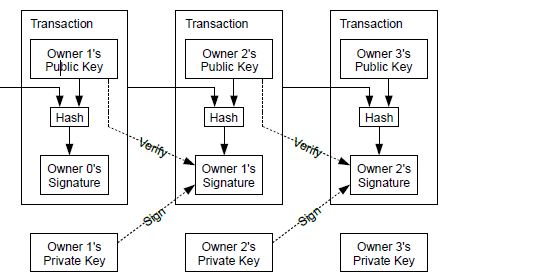
\includegraphics[trim = 0mm 0mm 30mm 0mm, width=120mm]{transaction}
\caption{Transaction}
\end{figure}

The problem of course is the payee can't verify that one of the owners did not double-spend
the coin. A common solution is to introduce a trusted central authority, or mint, that checks every
transaction for double spending. After each transaction, the coin must be returned to the mint to
issue a new coin, and only coins issued directly from the mint are trusted not to be double-spent.
The problem with this solution is that the fate of the entire money system depends on the
company running the mint, with every transaction having to go through them, just like a bank.
We need a way for the payee to know that the previous owners did not sign any earlier
transactions. For our purposes, the earliest transaction is the one that counts, so we don't care
about later attempts to double-spend. The only way to confirm the absence of a transaction is to
be aware of all transactions. In the mint based model, the mint was aware of all transactions and
decided which arrived first. To accomplish this without a trusted party, transactions must be
publicly announced [1], and we need a system for participants to agree on a single history of the
order in which they were received. The payee needs proof that at the time of each transaction, the
majority of nodes agreed it was the first received.

\section{Timestamp Server}

The solution we propose begins with a timestamp server. A timestamp server works by taking a hash of a block of items to be timestamped and widely publishing the hash, such as in a newspaper or Usenet post. The timestamp proves that the data must have existed at the time, obviously, in order to get into the hash. Each timestamp includes the previous timestamp in its hash, forming a chain, with each additional timestamp reinforcing the ones before it.

\begin{figure}[ht!]
\centering
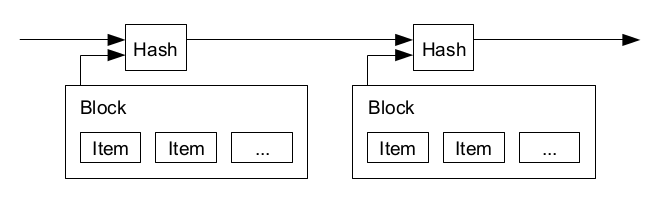
\includegraphics[trim = 0mm 0mm 0mm 0mm, width=120mm]{timestamp}
\caption{Timestamp Chain}
\end{figure}

\section{Proof-of-Work}

To implement a distributed timestamp server on a peer-to-peer basis, we will need to use a proof-of-work system similar to Adam Back's Hashcash, rather than newspaper or Usenet posts. The proof-of-work involves scanning for a value that when hashed, such as with SHA-256, the hash begins with a number of zero bits. The average work required is exponential in the number of zero bits required and can be verified by executing a single hash.
For our timestamp network, we implement the proof-of-work by incrementing a nonce in the block until a value is found that gives the block's hash the required zero bits. Once the CPU effort has been expended to make it satisfy the proof-of-work, the block cannot be changed without redoing the work. As later blocks are chained after it, the work to change the block would include redoing all the blocks after it.

\begin{figure}[ht!]
\centering
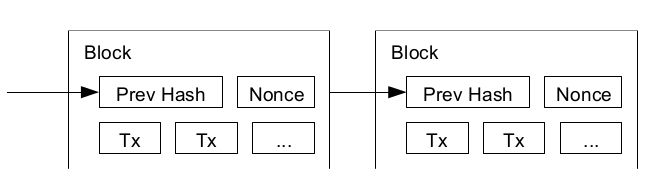
\includegraphics[trim = 0mm 0mm 0mm 0mm, width=120mm]{block_chain}
\caption{Block Chain}
\end{figure}

The proof-of-work also solves the problem of determining representation in majority decision making. If the majority were based on one-IP-address-one-vote, it could be subverted by anyone able to allocate many IPs. Proof-of-work is essentially one-CPU-one-vote. The majority decision is represented by the longest chain, which has the greatest proof-of-work effort invested in it. If a majority of CPU power is controlled by honest nodes, the honest chain will grow the fastest and outpace any competing chains. To modify a past block, an attacker would have to redo the proof-of-work of the block and all blocks after it and then catch up with and surpass the work of the honest nodes. We will show later that the probability of a slower attacker catching up diminishes exponentially as subsequent blocks are added.

To compensate for increasing hardware speed and varying interest in running nodes over time, the proof-of-work difficulty is determined by a moving average targeting an average number of blocks per hour. If they're generated too fast, the difficulty increases.

\section{Network}

The steps to run the network are as follows:
\begin{enumerate}
	\item New transactions are broadcast to all nodes.
	\item Each node collects new transactions into a block.
	\item Each node works on finding a difficult proof-of-work for its block
	\item When a node finds a proof-of-work, it broadcasts the block to all nodes.
	\item Nodes accept the block only if all transactions in it are valid and not already spent.
	\item Nodes express their acceptance of the block by working on creating the next block in the chain, using the hash of the accepted block as the previous hash.
\end{enumerate}

Nodes always consider the longest chain to be the correct one and will keep working on extending it. If two nodes broadcast different versions of the next block simultaneously, some nodes may receive one or the other first. In that case, they work on the first one they received, but save the other branch in case it becomes longer. The tie will be broken when the next proof- of-work is found and one branch becomes longer; the nodes that were working on the other branch will then switch to the longer one.

New transaction broadcasts do not necessarily need to reach all nodes. As long as they reach many nodes, they will get into a block before long. Block broadcasts are also tolerant of dropped messages. If a node does not receive a block, it will request it when it receives the next block and realizes it missed one.

\section{Incentive}

By convention, the first transaction in a block is a special transaction that starts a new coin owned by the creator of the block. This adds an incentive for nodes to support the network, and provides a way to initially distribute coins into circulation, since there is no central authority to issue them. The steady addition of a constant of amount of new coins is analogous to gold miners expending resources to add gold to circulation. In our case, it is CPU time and electricity that is expended.

The incentive can also be funded with transaction fees. If the output value of a transaction is less than its input value, the difference is a transaction fee that is added to the incentive value of the block containing the transaction. Once a predetermined number of coins have entered circulation, the incentive can transition entirely to transaction fees and be completely inflation free.

The incentive may help encourage nodes to stay honest. If a greedy attacker is able to assemble more CPU power than all the honest nodes, he would have to choose between using it to defraud people by stealing back his payments, or using it to generate new coins. He ought to find it more profitable to play by the rules, such rules that favour him with more new coins than everyone else combined, than to undermine the system and the validity of his own wealth.

\section{Reclaiming Disk Space}

Once the latest transaction in a coin is buried under enough blocks, the spent transactions before it can be discarded to save disk space. To facilitate this without breaking the block's hash, transactions are hashed in a Merkle Tree, with only the root included in the block's hash. Old blocks can then be compacted by stubbing off branches of the tree. The interior hashes do not need to be stored.

\begin{figure}[ht!]
\centering
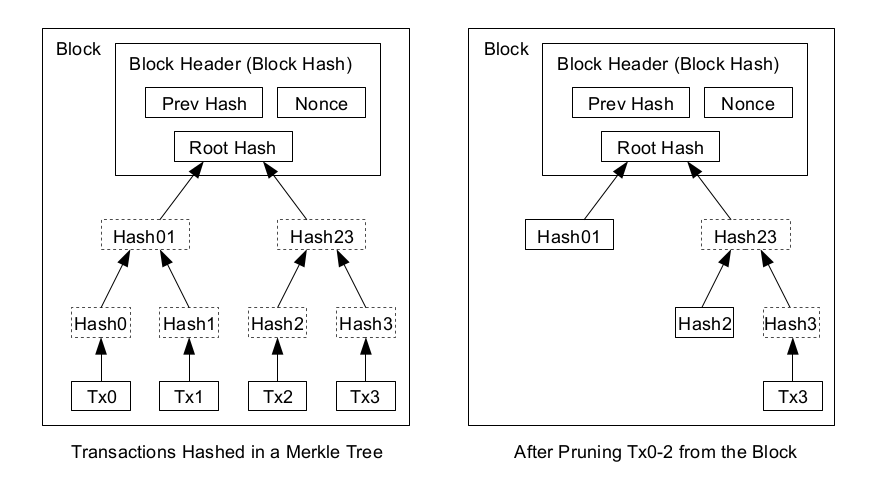
\includegraphics[trim = 0mm 0mm 0mm 0mm, width=120mm]{merkle_tree_and_pruning}
\caption{Transactions hashed in a Merkle Tree and pruning}
\end{figure}

A block header with no transactions would be about 80 bytes. If we suppose blocks are generated every 10 minutes, 80 bytes * 6 * 24 * 365 = 4.2MB per year. With computer systems typically selling with 2GB of RAM as of 2008, and Moore's Law predicting current growth of 1.2GB per year, storage should not be a problem even if the block headers must be kept in memory.

\section{Simplified Payment Verification}

It is possible to verify payments without running a full network node. A user only needs to keep a copy of the block headers of the longest proof-of-work chain, which he can get by querying network nodes until he's convinced he has the longest chain, and obtain the Merkle branch linking the transaction to the block it's timestamped in. He can't check the transaction for himself, but by linking it to a place in the chain, he can see that a network node has accepted it, and blocks added after it further confirm the network has accepted it.

\begin{figure}[ht!]
\centering
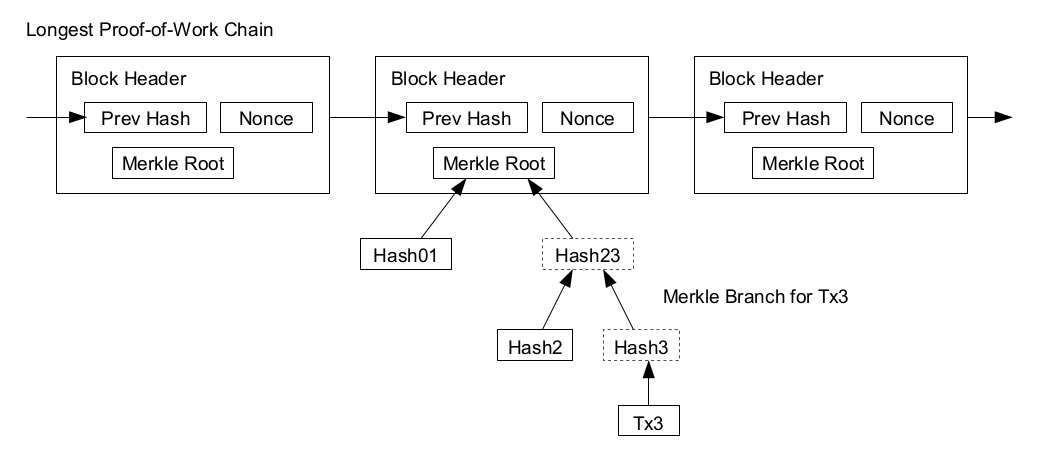
\includegraphics[trim = 0mm 0mm 0mm 0mm, width=120mm]{proof_of_work}
\caption{Proof-of-Work Chain}
\end{figure}

As such, the verification is reliable as long as honest nodes control the network, but is more vulnerable if the network is overpowered by an attacker. While network nodes can verify transactions for themselves, the simplified method can be fooled by an attacker's fabricated transactions for as long as the attacker can continue to overpower the network. One strategy to protect against this would be to accept alerts from network nodes when they detect an invalid block, prompting the user's software to download the full block and alerted transactions to confirm the inconsistency. Businesses that receive frequent payments will probably still want to run their own nodes for more independent security and quicker verification.

\section{Combining and Splitting Value}

Although it would be possible to handle coins individually, it would be unwieldy to make a separate transaction for every cent in a transfer. To allow value to be split and combined,transactions contain multiple inputs and outputs. Normally there will be either a single input from a larger previous transaction or multiple inputs combining smaller amounts, and at most two outputs: one for the payment, and one returning the change, if any, back to the sender.

\begin{figure}[ht!]
\centering
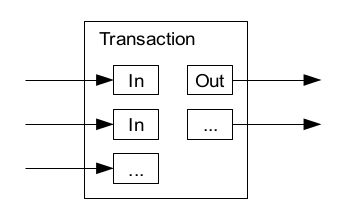
\includegraphics[trim = 0mm 0mm 0mm 0mm, width=70mm]{multiple_in_outs_transaction}
\caption{Inputs and Outputs in a transaction}
\end{figure}

It should be noted that fan-out, where a transaction depends on several transactions, and those transactions depend on many more, is not a problem here. There is never the need to extract a complete standalone copy of a transaction's history.

\section{Privacy}

The traditional banking model achieves a level of privacy by limiting access to information to the parties involved and the trusted third party. The necessity to announce all transactions publicly precludes this method, but privacy can still be maintained by breaking the flow of information in another place: by keeping public keys anonymous. The public can see that someone is sending an amount to someone else, but without information linking the transaction to anyone. This is similar to the level of information released by stock exchanges, where the time and size of individual trades, the \"tape\", is made public, but without telling who the parties were.

\begin{figure}[ht!]
\centering
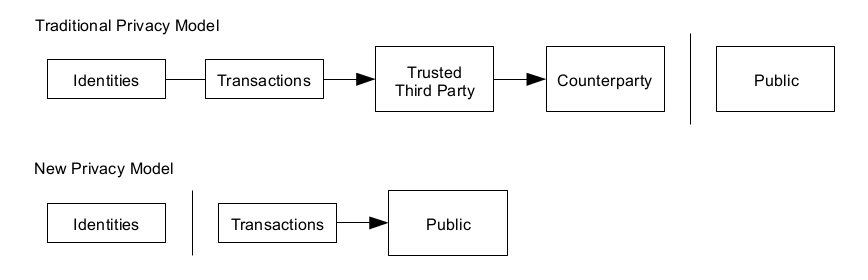
\includegraphics[trim = 0mm 0mm 0mm 0mm, width=120mm]{traditional_privacy_model}
\caption{Privacy Models}
\end{figure}

As an additional firewall, a new key pair should be used for each transaction to keep them from being linked to a common owner. Some linking is still unavoidable with multi-input transactions, which necessarily reveal that their inputs were owned by the same owner. The risk is that if the owner of a key is revealed, linking could reveal other transactions that belonged to the same owner.

\chapter{Under the Hood of the Bitcoin System}

Bitcoin is based on a peer-to-peer network layer that broadcasts data to all nodes on
the network. There are two types of object that are broadcast: transactions and blocks.
Both object types are addressed by a hash of the object data, and are broadcast through
the network to all nodes. Transactions are the operations whereby money is combined,
divided, and remitted. Blocks record the transactions vetted as valid.

\textbf{Spending.} Suppose that Alice wishes to remit 1 bitcoin to Bob and 2 to Carol. Alice’s
coins “reside” in prior transactions that designate her public key as beneficiary. To spend
coins, Alice creates a new transaction that endorses any such coins she has not spent
yet, e.g., she can endorse, using a digital signature, 4 coins each received from Diane
and Edgar as the inputs of her new transaction. As outputs she specifies 1 coin for Bob,
2 for Carol, and 4:99 of “change” back to herself. In this example, Alice chose to leave
a residual of 0:01 coin, which can be claimed as a fee by whoever vets it first.

\textbf{Vetting.} In order for a transaction to be confirmed, its various components must be
validated and checked against double spending. Once verified, transactions are incorporated
in frequently issued official records called blocks. Anyone is allowed to create
such blocks, and indeed two sorts of incentives are offered to attract verifiers to compete
for block creation: 
\begin{itemize}
	\item the collection of fees; and 
	\item the minting of new coins.
\end{itemize}

\textbf{Minting.} The bitcoin money supply expands as each block created may contain a special
generation transaction (with no explicit input) that pays the block creator a timedependent
amount for the effort (50 coins today, rapidly decreasing). The rate of block,
hence money, creation is limited by a proof of work of adaptive difficulty, that strives to
maintain a creation rate of one block every 10 minutes across the whole network. Bitcoin
transaction verification is thus a lucrative race open to all, but a computationally
expensive one. Note: “bad” blocks will be rejected by peers, invalidating their rewards.

\section{Transactions and Scripting: The Tools for Spending}
One of the main powers of the Bitcoin system is that the input and output of transactions
need not have a fixed format, but rather are constructed using a Forth-like stack-based
flexible scripting language. The transaction principals are not named users
but anonymous public keys, which users may freely create in any number they wish.

\textbf{Transactions.} Transaction encapsulate the movement of bitcoins by transfering the
value received from its inputs to its outputs (exception: generation transactions have
no explicit input at all). An input identifies a previous transaction output (as the hash
of the earlier transaction and an index to an output within it), and claims its full value.
An output specifies an amount; the outputs’ total must not exceed the inputs’. Both also
contain fragments of executable script, on the input side for redeeming inflows, and on
the output side for designating payees.

\textbf{Script fragments.} The scripting language is a Forth-like stack-based language. Operators
include cryptographic operations like SHA1 (which replaces the top item on the
stack with its hash), and CHECKSIG (which pops an ECDSA public key and signature
from the stack, verifies the signature for a “message” implicitly defined from the transaction
data, and leaves the result as a true or false on the stack). For a transaction to be
valid, its outputs must not exceed its inputs, and its issuer must show title to each input
claimed. Title is tested by evaluating the input script fragment concatenated with the
script fragment from the output (of an earlier transaction) that the input references.

\textbf{Standard transfer.} To illustrate how the stack-based scripting language can be used,
among other things, to designate and enforce the recipient of a transfer, we study the example
of the standard Bitcoin transaction used for transfer. To send coins to an address
stated as the hash of a public key, the payer, Alice, creates a transaction output with
the following associated script fragment (recall that since the amount is specified in a
special record associated with the output; the script only needs to enforce the recipient):

DUP HASH160 $\langle$recipient-address$\rangle$  EQUALVERIFY CHECKSIG        

The recipient, Bob, will notice the remittance (since it is broadcast to all), and mark it
for spending. Later on, to spend those received coins, he creates a transaction with an
input that redeems them, and an output that spends them. The redeeming input script is:

$\langle$signature$\rangle$ $\langle$public-key$\rangle$ 

Bob will have managed to spend coins received from Alice if his redemption is valid.
This is checked by executing the concatenated script ,the input fragment  pushes a signature and a key on the stack; the output fragment  checks that the key
hash matches the recipient, and checks the signature against transaction and key.

\section{Blocks and Coin Creation: the Process of Verifying}
Transactions become effective after they have been referenced in a block, which serve as
the official record of executed transactions. Transactions may only be listed in a block
if they satisfy such conditions as valid timestamping and absence of double spending.

\textbf{Blocks.} A block consists of one “coinbase” minting transaction, zero or more regular
spending transactions, a computational proof of work, and a reference to the chronologically
prior block. Thus the blocks form a singly linked blockchain, rooted in Nakamoto’s
genesis block whose hash is hardcoded in the software. The regular creation of new
blocks serves the dual purpose of ensuring the timely vetting of new transactions, and
the creation of new coins, all in a decentralized process driven by economic incentives
(the minting of new coins and the collection of fees) balanced by computational costs.
The difficulty of the required proof of work is adjusted by a feedback mechanism that
ensures an average block creation interval of 10 minutes across the entire network.

\textbf{Coinbase.} Currently, each new block may contain a coinbase transaction with an implicit
input value of 50 coins, with about 7M already minted as of this writing. The
minting rate is slated to decrease shortly, eventually to reach zero when the total supply
reaches about 21M bitcoins. The coinbase transaction also serves to claim all the fees in
the transactions collected in the block. Both minting and fees motivate people to create
blocks and hence keep the system alive.

\section{Forking and Conflict Resolution}
If two blocks are published nearly simultaneously, a fork in the chain can occur. Nodes
are programmed to follow the blockchain whose total proof-of-work difficulty is the
largest and discard blocks from other forks. Transactions on the discarded branch will
eventually be collected into blocks on the prevailing branch. This mechanism ensures
that one single ordering of transactions becomes apparent and accepted by all (although
it may take a few blocks’ time to become clear), and hence this solves the doublespending
problem.

\section{Theft or Loss of Bitcoins}
As all bitcoins are public knowledge (in the form of unredeemed transaction outputs),
what enables a user to spend a coin is possession of the associated private key. Theft or
loss of private keys, or signature forgeries, thus equate to loss of money in this world.

\subsection{Malware Attacks}
Reported malware attacks on Bitcoin are on the rise resulting in the theft of private
keys. The online wallet service mybitcoin.com recently lost \$1:3 million worth
of users’ coins due to malware. Several solutions can be envisaged Threshold cryptography. A natural countermeasure to malware is to split private keys into random shares, using standard threshold cryptography techniques and distribute
them onto multiple locations, e.g., a user’s desktop computer, her smart phone,
and an online service provider. In this way, only when a threshold number of these devices
collaborate, can a user spend her coins. Of course, doing so can harm the usability
of the system, since coins can no longer be spent without operating multiple devices
(even though not all the devices but only a chosen number of them are needed at once).
Super-wallets. To address the usability concern the simple idea of superwallet was purposed,
i.e., a user’s “personal bank” where most of her coins are stored. The superwallet
is split across multiple computing devices, using threshold techniques as above.
In addition, the user carries a small sub-wallet with her on her smartphone. Pre-approved
transactions are setup so that the user can withdraw money from her super-wallet onto
her sub-wallet, periodically in small amounts (similar to how real banks let people withdraw
cash from ATMs today). The user now only needs her smartphone to spend money
in her wallet, and in case her smartphone is captured by an adversary, the user only loses
the small amount of money that she has in her wallet, but not that in her personal bank.
Large amounts can always be spent from the super-wallet using a threshold of devices.
Both approaches can be implemented as backward-compatible and incrementally
deployable wrappers, requiring changes in the signature generation but not verification.

\subsection{Accidental Loss of Bitcoins}
Apart from malware, system failures or human errors can cause the accidental loss of the
wallet file (which stores the private keys needed to spend coins), which in turn leads to
the loss of coins (turning them into zombies). For example, bitomat, the third largest
bitcoin exchange, recently lost about \$200K worth of bitcoins (at the exchange rate at
the time) due to the loss of its private wallet file — the cause was later identified to be
human error, as the developer hosted the wallet on non-persistent cloud storage.

\textbf{Backups.} Naturally, the universal answer against accidental loss or adversarial destruction
of data, is to follow best-practice backup procedures. For backup purposes, the
wallet file should be treated like any other private cryptographic asset — meaning that
backups are a non-trivial proposition, not because of volume, but because of secrecy.
With Bitcoin, things are complicated by the incessant creation of keys.
Pseudo-random keys. To avoid having to back up a constantly growing wallet file,
a trivial solution is to generate all of one’s private keys not at random, but pseudorandomly
from a master secret that never changes, using a standard PRG. The problem
then reduces to that of backing up the short and static PRG seed, e.g., in a bank vault.
problem, of course, is that strong passwords are prone to memory loss and palimpsest.

\textbf{Offline (single-)password-based encryption.} One solution relies on the “optimal”
password-based encryption system of, which offers optimal trade-offs between password
strength (how tough it is to guess) and “snappiness” (how quickly it can be used,
which is also kept a secret). Users can even set multiple passwords with varying tradeoffs
for a common security goal: e.g., an everyday password, complex but snappy; and
a backup password, simple but just as secure by virtue of being made “sluggish”. A
pseudo-random wallet seed, encrypted à la, would combine static portability with
usable protection against both loss and theft, and is probably the best approach for an
isolated user who trusts his mental possessions more than his physical ones.

\textbf{Online (multi-)password-based encryption.} Another approach is to combine the power
of several memorable secrets into a single high-security “vault”, using the protocols of 
each member in some circle of friends holds a short totally private and long-term
memorable phrase. One member is a distinguished leader. Without revealing their secrets,
the members can perform private operations such as signing or decrypting a message
on behalf of the leader. With this protocol, a group of users can cooperate to let
the leader spend the coins from his wallet (kept as a public, static, accessible, encrypted
file), by issuing signatures on messages created by the leader. This approach provides
strong safety against loss, plus security against compromise of a subset of the group.

\textbf{Trusted paths.} Any of the above approaches can be combined with trusted-path devices,
which are dedicated hardware devices that let humans input and read out (tiny
amounts of) cryptographic data out of the reach of any malware. European banks use
the DigiPass, for example. Alas, while trusted-path protocols are well known and very
safe when it can be assumed that the remote server is uncorrupted (e.g., when talking
to a bank), in the Bitcoin case the server is the user’s own PC, possibly infected. It is an
interesting open problem to devise trusted-path protocols that are secure in this model,
when the trusted-path data is too tiny to provide cryptographic strength by itself.

\section{Scalability}
The smooth operation of Bitcoin relies on the timely broadcast of transactions and
blocks. A preprint  suggests that verifiers competing for the same reward have an
incentive to withhold the information needed to do so. However, since transactors have
an incentive to disseminate their data as quickly and widely as possible, not only is retention
futile, but economic forces will counter it by fostering circumvention services.

\subsection{Linear Transaction History}
The Bitcoin wallet software fetches the entire Bitcoin blockchain at installation,
and all new transactions and blocks are (supposedly) broadcast to all nodes.
The Bitcoin nodes cryptographically verify the authenticity of all blocks and transactions
as they receive them. Clearly, this approach introduces a scalability issue in the
longer term, in terms of both network bandwidth, and computational overhead associated
with cryptographic transaction verification. The scalability issue can be worrying
for smart phones with limited bandwidth, computational power, and battery supply.
The scalability issue can be addressed with a subscription-based filtering service.
Recall that Bitcoin nodes can be divided into broadly two classes, verifiers and clients.
Verifiers create new blocks and hence mint new coins. Verifiers are mostly nodes with
ample computational and bandwidth resources, typically desktop computers. By contrast,
clients are Bitcoin nodes that are not actively minting new coins, such as smart
phones. While verifiers have incentives to receive all transactions (to earn transaction
fees), clients may not care. In particular, all that is needed for clients to spend their
coins is that they receive transactions payable to their public key(s).

\textbf{Bitcoin filtering service.} Filtering service is a third-party cloud service provider
which filters Bitcoin transactions, and sends only relevant transactions to nodes that
have registered for the service. A Bitcoin client (e.g., a user’s smartphone) can send
a cryptographic capability to the filtering service, which allows the filtering service to
determine whether a transaction is payable to one or more of its public keys.

Identified the following desirable security and usability requirements are:

\begin{itemize}
	\item \textbf{Unlinkability without the capability.} While a user may allow the filtering service
to determine which transactions are payable to itself, no other party should be able
to link a user’s multiple public keys better than they can today (i.e., without the
filtering service).
	\item \textbf{Forward security.} The filtering service should be able to update its capability periodically,
such that in the case of compromise or a subpoena, the revealed capability
can allow one to identify new transactions targeted to a specific user, but cannot be
used to link the users’ transactions in the past.
	\item \textbf{Reasonable false positives and low false negatives.} A false positive is when the
filtering service mistakenly sends a user a non-relevant transaction. False positives
wastes a user’s bandwidth and computational power, but a user can locally detect
such false positives after receiving the transactions. A false negative is when the
filtering service fails to send a user a relevant transaction. The false negative rate
should ideally be 0.
\end{itemize}



\chapter{Bitcoin mining the hard way: The algorithms, protocols, and bytes}
\section{The purpose of mining}

Bitcoin mining is often thought of as the way to create new Bitcoins. But that's really just a secondary purpose. The primary importance of mining is to ensure that all participants have a consistent view of the Bitcoin data. Because Bitcoin is a distributed peer-to-peer system, there is no central database that keeps track of who owns Bitcoin. Instead, the log of all transactions is distributed across the network.
The main problem with a distributed transaction log is how to avoid inconsistencies that could allow someone to spend the same Bitcoins twice. The solution in Bitcoin is to mine the outstanding transactions into a block of transactions approximately every 10 minutes, which makes them official. Conflicting or invalid transactions aren't allowed into a block, so the double spend problem is avoided.
Although mining transactions into blocks avoid double-spending, it raises new problems: What stops people from randomly mining blocks? How do you decide who gets to mine a block? How does the network agree on which blocks are valid? Solving those problems is the key innovation of Bitcoin: mining is made very, very difficult, a technique called proof-of-work. It takes an insanely huge amount of computational effort to mine a block, but it is easy for peers on the network to verify that a block has been successfully mined. 
Each mined block references the previous block, forming an unbroken chain back to the first Bitcoin block. This block chain ensures that everyone agrees on the transaction record. It also ensures that nobody can tamper with blocks in the chain since re-mining all the following blocks would be computationally infeasible. As long as nobody has more than half the computational resources, mining remains competitive and nobody can control the block chain.
As a side-effect, mining adds new Bitcoin to the system. For each block mined, miners currently get 25 new Bitcoin (currently worth about \$15,000), which encourages miners to do the hard work of mining blocks. With the possibility of receiving \$15,000 every 10 minutes, there is a lot of money in mining.

\section{How mining works}
Mining requires a task that is very difficult to perform, but easy to verify. Bitcoin mining uses cryptography, with a hash function called double SHA-256. A hash takes a chunk of data as input and shrinks it down into a smaller hash value (in this case 256 bits). With a cryptographic hash, there's no way to get a hash value you want without trying a whole lot of inputs. But once you find an input that gives the value you want, it's easy for anyone to verify the hash. Thus, cryptographic hashing becomes a good way to implement the Bitcoin "proof-of-work".
In more detail, to mine a block, you first collect the new transactions into a block. Then you hash the block to form a 256-bit block hash value. If the hash starts with enough zeros, the block has been successfully mined and is sent into the Bitcoin network and the hash becomes the identifier for the block. Most of the time the hash isn't successful, so you modify the block slightly and try again, over and over billions of times. About every 10 minutes someone will successfully mine a block, and the process starts over.

The diagram below shows the structure of a specific block, and how it is hashed. The yellow part is the block header, and it is followed by the transactions that go into the block. The first transaction is the special coinbase transaction that grants the mining reward to the miner. The remaining transactions are standard Bitcoin transactions moving bitcoins around. If the hash of the header starts with enough zeros the block 
is successfully mined. For the block below, the hash is successful:0000000000000000e067a478024addfecdc93628978aa52d91fabd4292982a50 and the block became block \#286819 in the block chain.

\begin{figure}[ht!]
\centering
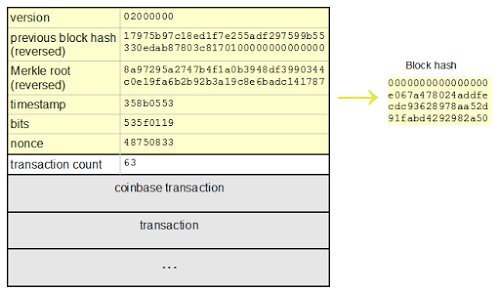
\includegraphics[trim = 0mm 0mm 0mm 0mm, width=120mm]{images/structure_of_bitcoin_block}
\caption{Structure of a Bitcoin}
\end{figure}

The block header contains a handful of fields that describe the block. The first field in the block is the protocol version. It is followed by the hash of the previous block in the block chain, which ensures all the blocks form an unbroken sequence in the block chain. (Inconveniently, the hash is reversed in the header.) The next field is the Merkle root a special hash of all the transactions in the block. This is also a key part of Bitcoin security, since it ensures that transactions cannot be changed once they are part of a block. Next is a (moderately accurate) timestamp of the block, followed by the mining difficulty value bits.  Finally, the nonce is an arbitrary value that is incremented on each hash attempt to provide a new hash value. The tricky part of mining is finding a nonce that works.

\section{Mining is very hard}
The difficulty of mining a block is astounding. At the current difficulty, the chance of a hash succeeding is a bit less than one in 1019. Finding a successful hash is harder than finding a particular grain of sand from all the grains of sand on Earth. To find a hash every ten minutes, the Bitcoin hash rate needs to be insanely large. Currently, the miners on the Bitcoin network are doing about 25 million gig hashes per second. That is, every second about 25,000,000,000,000,000 blocks gets hashed. I estimate (very roughly) that the total hardware used for Bitcoin mining cost tens of millions of dollars and uses as much power as the country of Cambodia.

Note that finding a successful hash is an entirely arbitrary task that doesn't accomplish anything useful in itself. The only purpose of finding a small hash is to make mining difficult, which is fundamental to Bitcoin security. It seems to me that the effort put into Bitcoin mining has gone off the rails recently.

Mining is funded mostly by the 25 Bitcoin reward per block, and slightly by the transaction fees (about 0.1 Bitcoin per block). Since the mining reward currently works out to about \$15,000 per block, that pays for a lot of hardware. Per transaction, miners are getting about \$34 in mining reward and \$0.10 in fees.

\section{Mining with a pool}
Since mining is so difficult, it is typically done in mining pools, where a bunch of miners share the work and share the rewards. If you mine by yourself, you might successfully mine a block and get 25 Bitcoin every few years. By mining as part of a pool, you could get a fraction of a Bitcoin every day instead, which for most people is preferable.

Mining pools use an interesting technique to see how much work miners are doing. They send out a block to be mined, and get updates from a miner whenever a miner gets a partial solution. Each partial solution proves the miner is working hard on the problem and gives the miner a share in the final reward when someone succeeds in mining the block.
For instance, if Bitcoin mining requires a hash starting with 15 zeroes, the mining pool can ask for hashes starting with 10 zeroes, which is a million times easier. Depending on the power of their hardware, a miner might find such a solution every few seconds or a few times an hour. Eventually one of these solutions will start with not just 10 zeroes but 15 zeroes, successfully mining the block and winning the reward for the pool. The reward is then split based on each miner's count of shares as a fraction of the total, and the pool operator takes a small percentage for overhead.

Most of the time someone outside the pool, will mine a block first. In that case, the pool operator sends out new data and the miners just start mining the new block. People in a pool can get edgy if a long time goes without a payout because of bad luck in mining.


\chapter{Limitations and Advantages}

\section{Challenges}
Despite the benefits that it presents, Bitcoin has some downsides
for potential users to consider. It has exhibited considerable
price volatility throughout its existence. New users are at risk of
improperly securing or even accidentally deleting their bitcoins
if they are not cautious. Additionally, there are concerns about
whether hacking could compromise the bitcoin economy.

\section{Volatility}
Bitcoin has weathered at least five significant price adjustments
since 2011.These adjustments resemble traditional speculative
bubbles: overoptimistic media coverage of Bitcoin prompts waves
of novice investors to pump up Bitcoin prices. The exuberance
reaches a tipping point, and the value eventually plummets.
Newcomer investors eager to participate run the risk of overvaluing
the currency and losing their money in a crash. Bitcoin’s fluctuating
value makes many observers skeptical of the currency’s
future.

Does this volatility foretell the end of Bitcoin? Some commentators
believe so. Others suggest that these fluctuations
are stress-testing the currency and might eventually decrease
in frequency as mechanisms develop to counteract volatility
If bitcoins were only used as stores of value or units of account,
the currency’s volatility could indeed endanger its future. It does
not make sense to manage business finances or keep savings in
bitcoins if the market price swings wildly and unpredictably.

When Bitcoin is used as a medium of exchange, however, vola -
tility is less of a problem Merchants can price their wares in
terms of a traditional currency and accept the equivalent number
of bitcoins. Customers who purchase bitcoins to make a one-time
purchase don’t care about what the exchange rate will look like
tomorrow; they simply care that Bitcoin can lower transaction
costs in the present. Bitcoin’s usefulness as a medium of exchange
might explain why the currency has grown more popular among
merchants in spite of its price volatility.It is also possible that
the value of bitcoins will become less volatile as more people
become familiar with the Bitcoin technology and develop realistic
expectations about its future.

\section{Security Breaches}
As a digital currency, Bitcoin presents some specific security challenges.
If people are not careful, they can inadvertently delete
or misplace their bitcoins. Once the digital file is lost, the money
is lost, just as with paper cash. If people do not protect their private
Bitcoin addresses, they can leave themselves open to theft.

Bitcoin wallets can now be protected by encryption, but users
must choose to activate the encryption. If a user does not encrypt
his or her wallet, bitcoins could be stolen through malware
Bitcoin exchanges, too, have at times struggled with security;
hackers successfully stole 24,000 BTC (\$250,000) from a bitcoin
exchange called Bitfloor in 2012 and mounted a massive series
of distributed denial-of-service (DDoS) attacks against the most
popular bitcoin exchange, Mt.Gox, in 2013. (Bitfloor eventually
repaid the stolen funds to its customers, and Mt.Gox ultimately
recovered from the DDoS attacks.) Of course, many of the security
risks facing Bitcoin are similar to those facing traditional currencies.
Dollar bills can be destroyed or lost, personal financial
information can be stolen and used by criminals, and banks can
be robbed or targeted by DDoS attacks.

Bitcoin users should take
care to learn about and prepare for security concerns just as they
currently do for other financial activities

\section{Criminal Uses}

There are also reasons for policymakers to be apprehensive
about some of Bitcoin’s exaptations. Because Bitcoin is pseudonymous,
policymakers and journalists have questioned whether
criminals can use it to launder money and accept payment for
illicit goods and services. Indeed, like cash, it can be used for ill
as well as for good.

For one example, we can look at the FBI taken down infamous Deep Web
black-market site known as “Silk Road.” Silk Road took advantage
of the anonymizing network Tor and the pseudonymous
nature of Bitcoin to make available a vast digital marketplace
where one can mail-order drugs and other licit and illicit wares.
Although Silk Road administrators never allowed the exchange
of any goods that resulted from fraud or harm, like stolen credit
card information or photographs of child exploitation, it did
allowed merchants to sell illegal products like forged identity documents
and illicit drugs. The pseudonymous nature of Bitcoin
allows buyers to purchase illegal goods online in the same way
that cash has been traditionally used to facilitate illicit purchases
in person. One study estimated the total monthly Silk Road
transactions amounted to be approximately \$1.2 million.

Bitcoin’s association with Silk Road has tarnished its reputation.
Following the publication of an article on Silk Road in 2011, senators Charles Schumer and Joe Manchin sent a letter
to Attorney General Eric Holder and the Drug Enforcement
Administration’s administrator Michele Leonhart calling for
a crackdown on Silk Road, the anonymizing software Tor, and
Bitcoin

Another concern is that Bitcoin can be used to launder money
for financing terrorism and trafficking in illegal goods. Although
these worries are currently more theoretical than evidential,
Bitcoin could indeed be an option for those who wish to discreetly
move ill-gotten money. Concerns about Bitcoin’s potential to
facilitate money laundering were stoked after Liberty Reserve, a
private, centralized digital-currency service based in Costa Rica,
was shut down by authorities on charges of money laundering.
While Liberty Reserve and Bitcoin appear similar because they
both provide digital currencies, there are important differences
between the two. Liberty Reserve was a centralized currency
service created and owned by a private company, allegedly for
the express purpose of facilitating money laundering. Bitcoin is
not. The transactions within the Liberty Reserve economy were
not transparent. Indeed, Liberty Reserve promised its customers
anonymity. Bitcoin, on the other hand, is a decentralized open
currency that provides a public record of all transactions. Money
launderers may attempt to protect their Bitcoin addresses and
identities, but their transaction records will always be public and
accessible at any time by law enforcement. Laundering money
through Bitcoin, then, can be seen as a much riskier undertaking
than using a centralized system like Liberty Reserve. Additionally, several bitcoin exchanges have taken steps to comply with anti–
money laundering record-keeping and reporting requirements.
The combination of a public ledger system and the cooperation of
bitcoin exchanges in collecting information on their customers
will likely make Bitcoin less attractive to launderers relative to
private anonymous virtual currencies.

It is also important to note that many of the potential down -
sides of Bitcoin are the same as those facing traditional cash.
Cash has historically been the vehicle of choice for drug traffickers
and money launderers, but policymakers would never
seriously consider banning cash. As regulators begin to contemplate
Bitcoin, they should be wary of the perils of overregulation.
In the worst-case scenario, regulators could prevent legitimate
businesses from benefitting from the Bitcoin network without
preventing money launderers and drug traffickers from using
bitcoins. If bitcoin exchanges are overburdened by regulation
and shut down, for instance, money launderers and drug traffickers
could still put money into the network by paying a person
in cash to transfer his or her bitcoins into their virtual wallets.
In this scenario, beneficial transactions are prevented by over -
regulation while the targeted activities are still able to occur.
The challenge for policymakers and regulators is how to develop
a system of oversight that assuages their twin concerns about
money laundering and illicit purchases without smothering the
benefits that Bitcoin is poised to provide to legitimate users in
their everyday lives.

\section{Benefits}

The first question that many people have when they learn
about Bitcoin is, Why would I want to use bitcoins when I can
use dollars? Bitcoin is still a new and fluctuating currency that
is not accepted by many merchants, so the uses for Bitcoin may
seem mostly experimental. To better understand why people
might want to use Bitcoin, it helps to think of it, not necessarily
as a replacement for traditional currencies, but rather as a new
payments system.

\subsection{Lower Transaction Costs}

Because there is no third-party intermediary, Bitcoin transactions
are substantially cheaper and quicker than traditional payment
networks. And because transactions are cheaper, Bitcoin makes
micropayments and other innovations possible. Additionally,
Bitcoin holds much promise as a way to lower transaction costs
for small businesses and global remittances, alleviate global poverty
by improving access to capital, protect individuals against
capital controls and censorship, ensure financial privacy for
oppressed groups, and spur innovation (within and on top of the
Bitcoin protocol). On the other hand, Bitcoin’s decentralized
nature also presents opportunities for crime. The challenge, then,
is to develop processes that diminish the opportunities for criminality
while maintaining the benefits that Bitcoin can provide.

First, Bitcoin is attractive to cost-conscious small businesses
looking for ways to lower the transaction costs of doing business.
Credit cards have greatly expanded the ease of transacting, but
their use comes with considerable costs to merchants. Businesses
that wish to offer the option of credit card payments to their customers
must first pay for a merchant account with each credit
card company. Depending on the terms of agreement with each
credit card company, businesses must then pay a variety of
authorization fees, transaction fees, statement fees, interchange
fees, and customer-service fees, among other charges. These fees quickly add up and significantly increase the cost of doing business.
However, if a merchant neglects to accept credit card payments
to save on fees, he or she could lose a considerable amount
of business from customers who enjoy the ease of credit cards.
Since Bitcoin facilitates direct transactions without a third
party, it removes costly charges that accompany credit card transactions.
The Founders Fund, the venture capital fund headed by
Peter Thiel of PayPal and Facebook fame, recently invested \$3
million in the payment-processing company BitPay because of
the service’s ability to lower the costs of doing online commerce
across borders.19 In fact, small businesses have already started
to accept bitcoins as a way to avoid the costs of doing business
with credit card companies.20 Others have adopted the currency
for its speed and efficiency in facilitating transactions.21 Bitcoin
will likely continue to lower transaction costs for businesses that
accept it as more people adopt the currency.

Accepting credit card payments also puts businesses on the
hook for charge-back fraud. Merchants have long been plagued by
fraudulent “charge-backs,” or consumer-initiated payment reversals
based on a false claim that a product has not been delivered.
Merchants therefore can lose the payment for the item and the
item itself, and also have to pay a fee for the charge-back. As a
nonreversible payment system, Bitcoin eliminates the “friendly
fraud” wrought by the misuse of consumer charge-backs. This can
be very important for small businesses.

Consumers like charge-backs, however, because that system
protects them from unscrupulous merchants or merchant errors.
Consumers may also enjoy other benefits that merchant-account
fees help fund. Indeed, many consumers and merchants will probably
stick to traditional credit card services even if Bitcoin payments
become available. Still, the expanded choices in payment
options would benefit people of all preferences.
Those who want the protection and perks of using a credit
card can continue to do so, even if they pay a little more. Those
who are more price- or privacy-conscious can use bitcoins
instead. Not having to pay merchant fees means that merchants
who accept Bitcoin have the option to pass the savings on to consumers.
That is the business model of the Bitcoin Store,23 which
sells thousands of consumer electronics at discounted prices and
only accepts bitcoins. The same Samsung Galaxy Note tablet that
sells on Amazon for \$779 plus shipping24 sells at the Bitcoin Store
for a mere \$480.25 In this way, Bitcoin provides more low-cost
options to bargain hunters and small businesses without detracting
from the traditional credit card services that some consumers
prefer.

As an inexpensive funds-transfer system, Bitcoin also holds
promise for the future of low-cost remittances. In 2012, immigrants
to developed countries sent at least \$401 billion in remittances
back to relatives living in developing countries. The
amount of remittances is projected to increase to \$515 billion
by 2015.27 Most of these remittances are sent using traditional
brick-and-mortar wire services such as Western Union and
MoneyGram, which charge steep fees for the service and can take
several business days to transfer the funds.28 In the first quarter of
2013, the global average fee for sending remittances was 9.05 percent.
29 In contrast, transaction fees on the Bitcoin network tend
to be less than 0.0005 BTC,30 or 1 percent of the transaction. This
entrepreneurial opportunity to improve money transfers has
attracted investments from big-name venture capitalists. Even
MoneyGram and Western Union are contemplating whether to
integrate Bitcoin into their business models. Bitcoin allows for
instantaneous, inexpensive remittances, and the reduction in the
cost of global remittances for consumers could be considerable.

\subsection{Potential to Combat Poverty and Oppression}

Bitcoin also has the potential to improve the quality of life for the
world’s poorest. Improving access to basic financial services is a
promising antipoverty technique. According to one estimate,
64 percent of people living in developing countries lack access to
these services, perhaps because it is too costly for traditional financial
institutions to serve poor, rural areas Because of the impediments
to developing traditional branch banking in poor areas,
people in developing countries have turned to mobile banking services
for their financial needs. The closed-system mobile payment
service M-Pesa has been particularly successful in countries such
as Kenya, Tanzania, and Afghanistan. Entrepreneurs are already
moving to this model; the Bitcoin wallet service Kipochi recently
developed a product that allows M-Pesa users to exchange bitcoins.
Mobile banking services in developing countries can be
further augmented by the adoption of Bitcoin. As an open-system
payment service, Bitcoin can provide people in developing countries
with inexpensive access to financial services on a global scale.
Bitcoin might also provide relief to people living in countries
with strict capital controls. The total number of bitcoins
that can be mined is capped and cannot be manipulated. There
is no central authority that can reverse transactions or prevent
the exchange of bitcoins between countries. Bitcoin therefore
provides an escape hatch for people who desire an alternative
to their country’s devalued currencies or frozen capital markets.
We have already seen examples of people turning to Bitcoin to
evade the harmful effects of capital controls and central-bank
mismanagement. Some Argentines, for instance, have adopted
Bitcoin in response to the country’s dual burdens of a 25 percent
inflation rate and strict capital controls. Demand for bitcoins is
so strong in Argentina that one popular bitcoin exchange is planning
to open an Argentine office. Argentine Bitcoin use continues
to surge in the face of Argentina’s capital mismanagement.

Individuals in oppressive or emergency situations might
also benefit from the financial privacy that Bitcoin can provide.
There are many legitimate reasons why people seek privacy in
their financial transactions. Spouses fleeing abusive partners
need some way to discreetly spend money without being tracked.
People seeking controversial health services desire financial privacy
from family members, employers, and others who might
judge their decisions. Recent experiences with despotic
governments suggest that oppressed citizens would benefit greatly from
the ability to make private transactions free from the grabbing
hands of tyrants. Bitcoin provides some of the privacy that has
traditionally been afforded through cash—with the added convenience
of digital transfer.

\subsection{Stimulus for Financial Innovation}
One of the most promising applications of Bitcoin is as a platform
for financial innovation. The Bitcoin protocol contains the digital blueprints for a number of useful financial and legal services
that programmers can easily develop. Since bitcoins are, at
their core, simply packets of data, they can be used to transfer,
not only currencies, but also stocks, bets, and sensitive information.
Some of the features that are built into the Bitcoin protocol
include micropayments, dispute mediations, assurance contracts,
and smart property. These features would allow for the easy
development of Internet translation services, instantaneous processing
for small transactions (like automatically metering Wi-Fi
access), and Kickstarter-like crowdfunding services.
Additionally, programmers can develop alternative protocols
on top of the Bitcoin protocol in the same way that the Web
and email are run on top of the Internet’s TCP/IP protocol. One
programmer has already proposed a new protocol layer to add
on top of the Bitcoin protocol that can improve the network’s
stability and security. Another programmer created a digital
notary service to anonymously and securely store a “proof of
existence” for private documents on top of the Bitcoin protocol.
Other programmers have adopted the Bitcoin model as a way to encrypt email communications. Another group of developers
has outlined an add-on protocol that will improve the privacy
of the network. Bitcoin is thus the foundation upon which
other layers of functionality can be built. The Bitcoin project can
be best thought of as a process of financial and communicative
experimentation. Policymakers should take care that their directives
do not quash the promising innovations developing within
and on top of this fledgling protocol.

\chapter{Conclusion}

Bitcoin is an exciting innovation that has the potential to
greatly improve human welfare and jump-start beneficial and
potentially revolutionary developments in payments, communications,
and business. Bitcoin’s clever use of public-key encryption
and peer-to-peer networking solves the double-spending
problem that had previously made decentralized digital currencies
impossible. These properties combine to create a payment
system that could lower transactions costs in business and remittances,
alleviate poverty, provide an escape from capital controls
and monetary mismanagement, allow for legitimate financial
privacy online, and spur new financial innovations. On the other
hand, as “digital cash,” Bitcoin can be used for money laundering
and illicit trade. Banning Bitcoin is not the solution to ending
money laundering and illicit trade, just as banning cash is not a
solution to these same ills.

Bitcoin could ultimately fail as an experimental digital currency
and payment system. An unanticipated problem could arise and
undermine the bitcoin economy. A superior cryptocurrency could
outcompete and replace Bitcoin. It could simply fizzle out as a fad.
The possibilities for failure are endless, but one reason for failure
should not be that policymakers did not understand its workings
and potential. We are ultimately advocating not for Bitcoin, but
for innovation. It is important that policymakers allow this experimentation
to continue. Policymakers should work to clarify how
Bitcoin is regulated and to normalize its regulation so that we have
the opportunity to learn just how innovative Bitcoin can be.
%
% Continue adding new chapters, sections and 
% subsections.
%
% ***   Creating Bibliography   ***
%
% Do not delete the following two lines
%
\clearpage
\addcontentsline{toc}{chapter}{\quad Bibliography}
%
% The markups for creating the bibliography begins here.
% One sample bibliography item is included. 
% Add additional items if there are any.
%
\begin{thebibliography}{99}
\bibitem{First}
Nakamoto, Satoshi (2012) {\em Bitcoin: A peer-to-peer electronic cash system, 2009}, \url{http://www.bitcoin.org/bitcoin.pdf}
\bibitem{Second}
Reid, F.  and  Harrigan, M. {\em  An  Analysis  of  Anonymity  in  the  Bitcoin System},(2011, Oct). 1318-1326
\bibitem{Third}
Lowenthal, Thomas. {\em Bitcoin: inside the encrypted, peer-to-peer digital currency.} Ars Technica. Retrieved 14 (2011).
\bibitem{Fourth}
Barber, Simon, et al. {\em Bitter to better—how to make bitcoin a better currency.} Financial Cryptography and Data Security. Springer Berlin Heidelberg, (2012). 399-414.
\bibitem{Fifth}
Grinberg, Reuben. {\em Bitcoin: an innovative alternative digital currency.} (2012).
\bibitem{Sixth}
Brito, Jerry, and Andrea Castillo.{\em Bitcoin: A Primer for Policymakers.} Mercatus Center: Geroge Mason University. \url{http://mercatus.org/sites/default/files/Brito_BitcoinPrimer_embargoed.pdf} (2013).
\end{thebibliography}
%
% Printing the last page
%
%
\newpage
\thispagestyle{empty}
\vspace*{\fill}
\begin{flushright}

\includegraphics{VidyaLogo}\\[0.5cm]
{\Large \bf \sf  Department of Computer Science and Engineering}\\
{\sf Vidya Academy of Science \& Technology\\
Thalakkottukara, Thrissur - 680 501\\
({\tt http://www.vidyaacademy.ac.in})}
\end{flushright}
%
%
%   ***   The end   ***
%
\end{document}
